\chapter{Algoritmi euristici}
In questo capitolo verranno trattati algoritmi euristici che non fanno uso di CPLEX. La necessità di non utilizzare CPLEX si ha per istanze con un numero elevato di nodi (10000-20000 nodi).\\
Per queste istanze la risoluzione del tableau attraverso CPLEX diventerebbe molto un'operazione molto onerosa per via dell'alto numero di variabili che verrano create e su cui verrà svolro il calcolo.\\
Attraverso gli algoritmi euristici, viene computata un'approssimazione della soluzione ottima e spesso però può essere sfruttata inizialmente dal risolutore CPLEX. Ad esempio questo può essere aggiunta prima della computazione, utilizzando la funzione \textit{CPXaddmipstarts()}, o ,se già definita, può essere modificata tramite \textit{CPXchgmipstarts()}.

\section{Euristici di costruzione}
Questa prima tipologia di algoritmi euristici è necessaria per la computazione di una prima soluzione ammissibile del problema.
\subsection{Nearest Neighborhood}
Questo algoritmo è basato su un approccio di tipo greedy.
L'algoritmo sceglie un nodo generico tra quelli che compongono il grafo. In seguito, iterativamente seleziona degli archi del grafo secondo il criterio enunciato nella seguente parte.\\
All'iterazione i-esima, vengono analizzati i costi degli archi che hanno un estremo pari al nodo selezionato all'iterazione i-1.\\
Viene selezionato l'arco che tra questi ha costo minore e il nuovo nodo raggiunto viene impostato come punto di partenza per analizzare i costi degli archi all'iterazione successiva (vedi Figura \ref{nearest_neighborhood}). All'ultima iterazione viene scelto l'arco che collega l'ultimo nodo visitato al nodo scelto inizialmente.\\
Il problema di questo algoritmo è che in ogni iterazione viene selezionato esclusivamente il vertice più vicino a quello scelto precedentemente, senza però prevedere la futura evoluzione del ciclo, creato dall'algoritmo.\\
Come in Figura \ref{nearest_neighborhood}, la scelta dell'arco di costo minimo non implica che in seguito venga generata la soluzione ottima. Scegliendo un nodo iniziale differente, viene generato un tour differente.\\
Definito \textbf{n} come il numero di nodi presenti nel grafo, si avranno quindi n soluzioni differenti, ottenute ciascuna attraverso n iterazioni dell'algoritmo. In seguito tra queste possibli soluzioni, verrà selezionata quella di costo minore.\\
\begin{figure}[h] 
\begin{center} 
  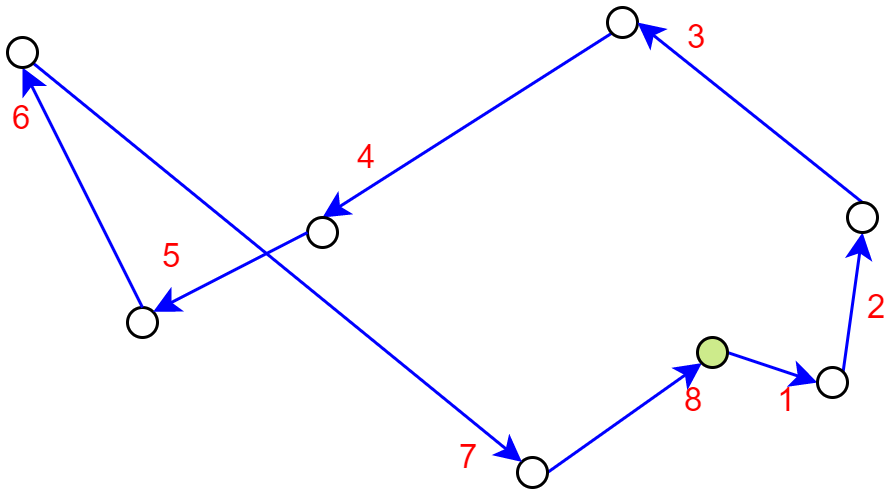
\includegraphics[scale=0.4]{Images/nearest_neighborhood}\\ 
  \caption{\footnotesize{Esempio di esecuzione di Nearest Neighborhood.}}
  \label{nearest_neighborhood} 
\end{center} 
\end{figure}
Per migliorare l'algoritmo viene aggiunta una scelta aleatoria, utilizzando il metodo Greedy Adaptive Search Procedure (GASP). Ad ogni iterazione, invece di selezionare l'arco di costo minimo, vengono messi in evidenza i tre archi con costo minore e ne viene selezionato casualmente uno tra questi.\\
Un'implementazione alternativa invece fa uso sia del metodo standard che del metodo GASP. In questo caso la scelta casuale non viene fatta su ogni iterazione ma con una certa periodicità fissata inizialmente.

\subsection{Heuristic Insertion}
L'algoritmo seguente usa un approcco simile al precedente ma prevede la selezione di un ciclo iniziale a cui apportare modifiche, per ottenere una soluzione iniziale ammissibile del problema. Per definire il ciclo di partenza vengono utilizzati diversi metodi. Di seguito sono riportati i due più utilizzati:
\begin{itemize}
\item{\textbf{Selezione di due nodi}\\
Vengono scelti i due nodi più lontani tra loro nel grafo o due nodi casuali e  sono selezionati i due archi orientati che li collegano.
}
\item{\textbf{Inizializzazione geometrica}\\
Nel caso in cui i nodi siano punti 2D, può essere calcolata la convex-hull e utilizzarla come ciclo iniziale. 
}
\end{itemize}
In seguito a tale operazione, questa soluzione viene modificata iterativamente. Per ogni coppia di nodo non appartenente al ciclo \textbf{C}, restituito dall'iterazione precedente, viene calcolato l'extramileage $\Delta_h$ come segue:
$$\Delta_h = \underset{(a,b)\in C}{min} c_{ah}+c_{hb}-c_{ay}$$
con $c_ij$ costo dell'arco che collega i a j (vedi Figura \ref{partial_cycle}).\\
Alla fine di ciascuna iterazione viene aggiunto nel grafo il nodo \textbf{k} che minimizza l'\textbf{extramileage} (vedi Figura \ref{insertion}):\\
$$k = arg\underset{h}{min}\Delta_{h}$$
Un modo per aggiungere aleatorietà a questo algoritmo può essere quello di sfruttare l'approccio GASP nella selezione del minimo extramileage. Il nodo da aggiungere in un'iterazione al grafo, viene selezionato in modo casuale tra i tre con $\Delta$ minore.
\begin{figure}[h] 
\begin{center} 
  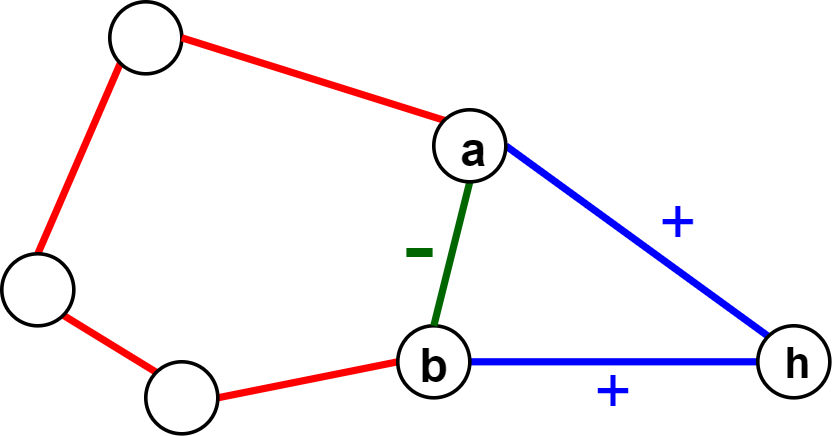
\includegraphics[scale=0.2]{Images/partial_cycle}\\ 
  \caption{\footnotesize{Parte del calcolo dell'extramileage del nodo \textbf{h}.}}
  \label{partial_cycle}
\end{center}
\end{figure}
\begin{figure}[h] 
\begin{center} 
  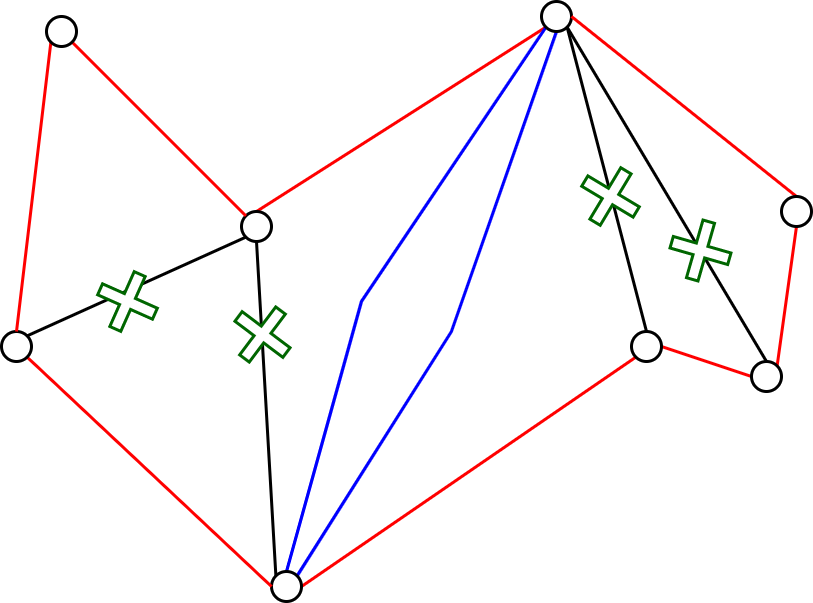
\includegraphics[scale=0.4]{Images/insertion}\\ 
  \caption{\footnotesize{Esempio dell'applicatione di Heuristic insertion.}}
  \label{partial_cycle}
\end{center}
\end{figure}